% Chapter 1: Introduction

\chapter{Introducción} % Main chapter title

\label{Chapter1}

%-------------------------------------------------------------------------------

% Define some commands to keep the formatting separated from the content
\newcommand{\keyword}[1]{\textbf{#1}}
\newcommand{\tabhead}[1]{\textbf{#1}}
\newcommand{\code}[1]{\texttt{#1}}
\newcommand{\file}[1]{\texttt{\bfseries#1}}
\newcommand{\option}[1]{\texttt{\itshape#1}}
\newcommand{\Mod}[1]{\ (\mathrm{mod}\ #1)}

%-------------------------------------------------------------------------------
En este capítulo se presenta la motivación del problema, los conceptos previos que ayudarán al lector a entender mejor el desarrollo, siguiendo con la definición del problema y, por último, se muestra una revisión del estado del arte relacionado con este.

\section{Estructura de la memoria}
La memoria de este trabajo final de grado se estructura de la siguiente manera:
\begin{itemize}
	\item Capítulo 1, en este capítulo se introduce el tema a tratar, describiendo el problema y el estado del arte de este, así como conceptos previos relacionados.
	\item Capítulo 2, en este capítulo se muestran los objetivos que se esperan alcanzar con este trabajo final de grado.
	\item Capítulo 3, en este capítulo se describe de manera algorítmica la metaheurística empleada para abordar el problema tratado.
	\item Capítulo 4, en este capítulo se explica el desarrollo de las funciones para obtener una solución al problema.
	\item Capítulo 5, en este capítulo se exponen los resultados recopilados durante el procesamiento del problema, así como el análisis de estos.
	\item Capítulo 6, en este capítulo se muestran las conclusiones obtenidas durante todo este trabajo final de grado.
\end{itemize}

\section{Motivación del problema}

En la actualidad, los datos se han convertido en una pieza fundamental en la vida cotidiana de las personas. Tanto su obtención como su posterior tratamiento son grandes retos que deben ser estudiados y, por supuesto, realizar esto de una manera eficiente y en el menor tiempo posible, es un reto aún mayor. A partir de esto se obtiene el término grafo, el cual es fundamental en este ámbito y que se define como la relación entre nodos o vértices mediante uniones llamadas aristas, y esto, es lo realmente interesante a estudiar, las relaciones existentes entre los distintos nodos.\newline
Existen muchos casos en los que se puede realizar la obtención y tratamiento de estos datos, como, por ejemplo, la red social Facebook\footnote{https://es-es.facebook.com/}, que como se observa en la figura \ref{fig:facebook-graph} define su grafo como las relaciones entre las personas y aficiones que les unen. Además, ofrece una \gls{API} \footnote{Conjunto de métodos que forman parte de una librería y que a modo de capa de abstracción son publicados para que puedan ser usados en otros desarrollos software.} con la que poder interactuar con los datos que son recopilados en ella \cite{api-graph}.

 \begin{figure}[H]
	\centering
	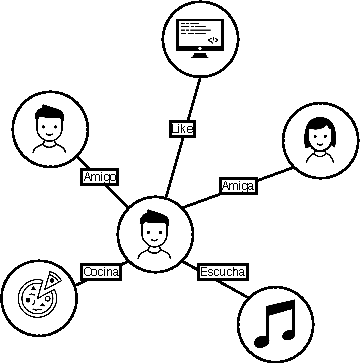
\includegraphics[scale=0.8]{Figures/facebook-graph.pdf}
	\caption{Grafo de relaciones en Facebook.}
	\label{fig:facebook-graph}
\end{figure}

Por otro lado, también muy cercano a la vida cotidiana de las personas, se encuentran las redes de telecomunicaciones, figura \ref{fig:teleco-graph}, que interconectan todos los aparatos electrónicos, que de una manera u otra se comunicación entre ellos, y las redes de metro, figura \ref{fig:metro-graph}, que permiten el movimiento de las personas en la ciudad y pueden ser estudiadas por uso, localización, etcétera.

\begin{figure}[H]
	\begin{minipage}[b]{0.5\linewidth}
			\centering
			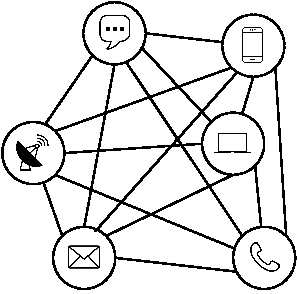
\includegraphics[scale=0.8]{Figures/teleco-graph.pdf}
			\caption{Grafo de telecomunicaciones.}
			\label{fig:teleco-graph}
	\end{minipage}
	\begin{minipage}[b]{0.5\linewidth}
		\centering
		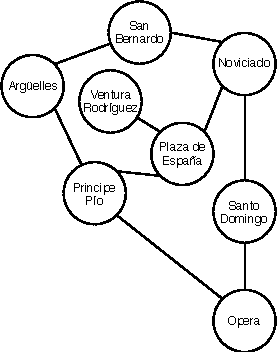
\includegraphics[scale=0.8]{Figures/metro-graph.pdf}
		\caption{Grafo sección del metro de Madrid.}
		\label{fig:metro-graph}
	\end{minipage}
\end{figure}

Y, por último, otra representación de grafo es el de las moléculas y los enlaces químicos \cite{grafo-molecula}, que se pueden representar como en la figura \ref{fig:molecula-graph}.

 \begin{figure}[H]
	\centering
	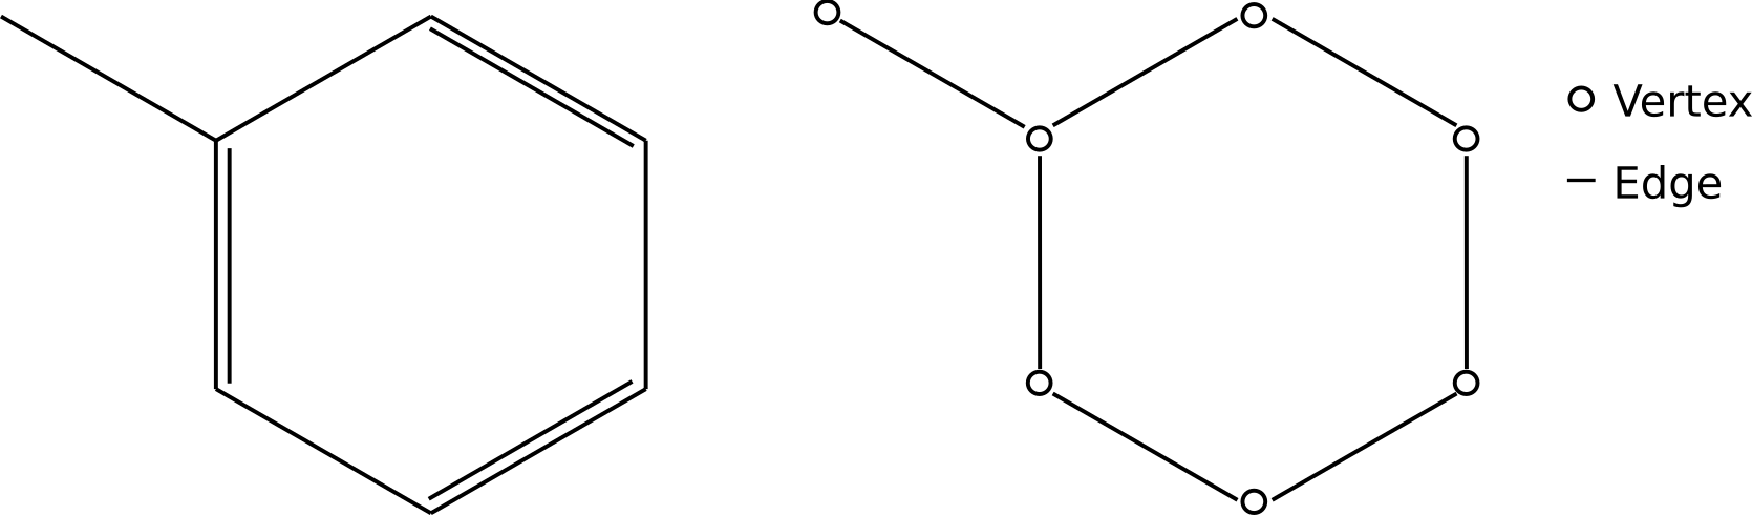
\includegraphics[scale=0.3]{Figures/molecula-graph.pdf}
	\caption{Representación estándar y en grafo de la molécula del Tolueno.}
	\scriptsize Fuente: https://www.blopig.com/blog/2019/01/graph-based-methods-for-cheminformatics
	\label{fig:molecula-graph}
\end{figure}

Estos ejemplos, tienen en común las conexiones entre todos los nodos que forman su estructura de grafo, y son muchas las aplicaciones e información que se obtiene de ellos como, nuevas terapias \cite{top-molec}, visión computacional y reconocimiento de patrones \cite{mcp-compVision}, análisis del mercado bursátil para conocer nuevas formas de predicción de éxito en inversiones \cite{vid-graf-ai}.

Por todo esto, es muy importante tratar los datos de forma adecuada y responsable, así como las relaciones entre ellos eficientemente. Para ello se han creado incluso base de datos orientadas a grafos, como es el caso de Neo4j \footnote{https://neo4j.com/}, con el fin de entender las relaciones y así poder hallar nuevas técnicas y más posibilidades para afrontar problemas y resolverlos de una manera mucho más ágil.


\section{Conceptos previos}
Para comprender mejor todas las explicaciones que se van a exponer a lo largo del documento, se describen a continuación los conceptos más importantes.

\subsection{Optimización combinatoria}
La optimización combinatoria es el área, dentro de las matemáticas aplicadas, que se encarga de maximizar o minimizar una función en un espacio de soluciones, el cuál debe ser finito. Los problemas que pertenecen a esta área tienen en común la dificultad de encontrar soluciones factibles, puesto que existen muchas posibles y alguna de estas es óptima.\\
Algunos casos conocidos son el problema de la mochila\footnote{https://www.sciencedirect.com/topics/computer-science/knapsack-problem} o el problema del vendedor viajero\footnote{https://www.sciencedirect.com/topics/computer-science/travelling-salesman-problem}. Estos problemas tienen un planteamiento sencillo, pero son difíciles de solucionar, y mediante ciertos algoritmos, como se explicará en la sección \ref{sec:heu-meta}, se pueden obtener soluciones factibles en tiempos de cómputo reducidos.\\
En la actualidad es un campo con un gran crecimiento ya que ``muchos de los problemas de la vida real pueden ser formulados mediante optimización combinatoria'' \cite{opt-comb-rg}.

\subsection{Heurística y Metaheurística}
\label{sec:heu-meta}
Se define heurística, según el Diccionario de la Real Academia de la Lengua Española, como ``técnica de la indagación y del descubrimiento'' y ``en algunas ciencias, manera de buscar la solución de un problema mediante métodos no rigurosos, como por tanteo, reglas empíricas etc.''\cite{rae-heuristica}. Aplicándolo a temas científicos se define como el proceso de creación de medios, estrategias y principios para alcanzar un objetivo eficaz al problema dado \cite{conceptodef-heuristica}. El término heurística fue acuñado por George Polya en su libro ``How to Solve It'' \cite{gpolya-book-1}, más tarde traducido a ``Cómo plantear y resolver problemas'' \cite{gpolya-book-2}.

Añadiendo al término heurística el prefijo ``meta'', procedente del griego que significa ``más allá'' o ``nivel superior'', se puede definir metaheurística como el conjunto de procedimientos heurísticos combinados para obtener una solución a un problema que no tiene un algoritmo heurístico específico o su aplicación es ineficiente \cite{wiki-metaheuristica}. Este término lo acuñó Fred Glover en sus trabajos sobre búsqueda tabú en 1986 \cite{fred-glover}.

Existen una gran variedad de algoritmos metaheurísticos que se pueden clasificar de diferentes maneras según el enfoque, en la figura \ref{fig:clasif-metahs} se muestra una posible clasificación.

\begin{figure}[H]
	\centering
	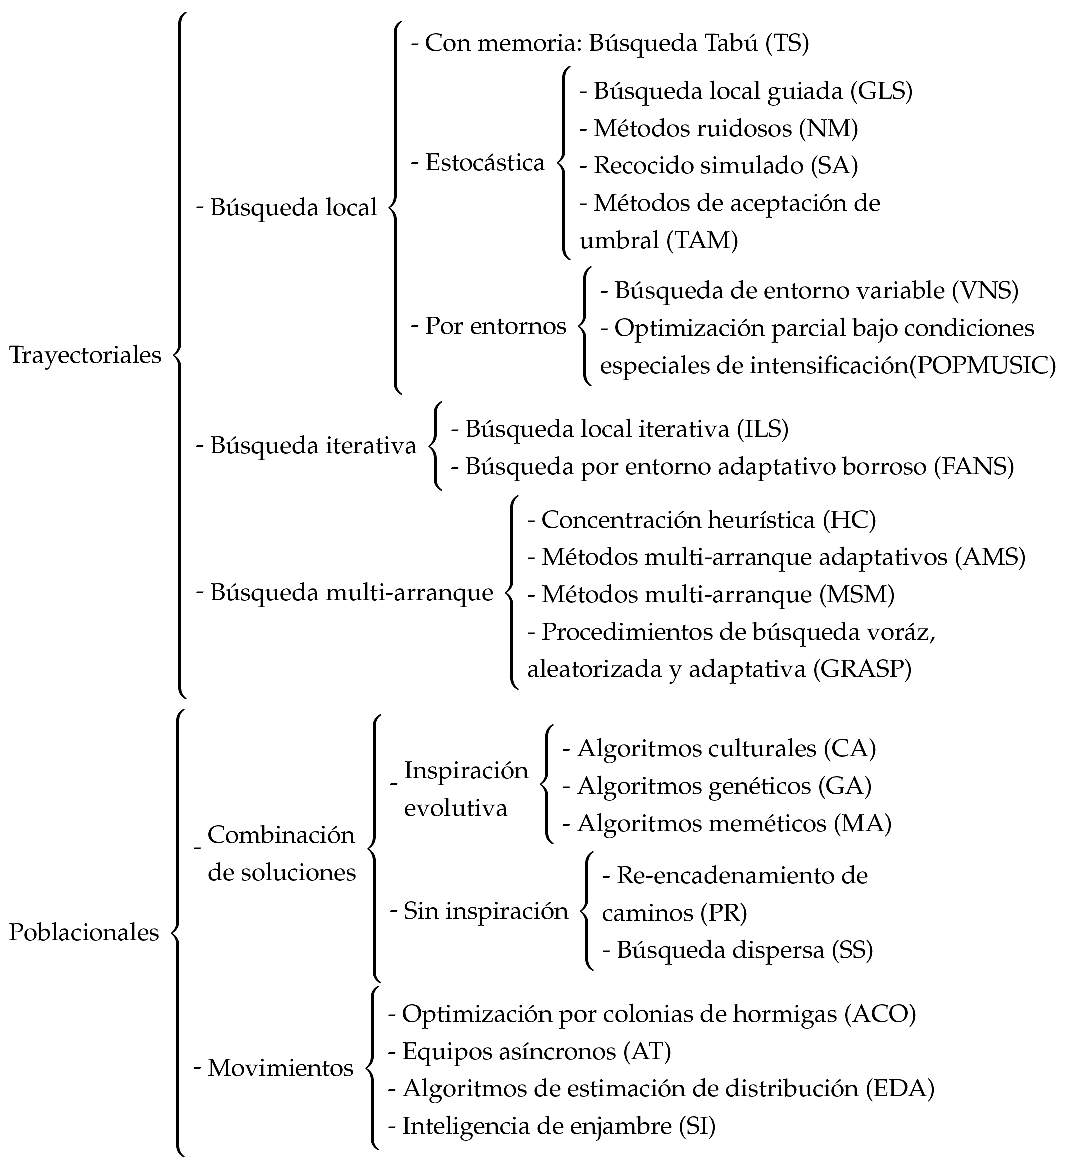
\includegraphics[scale=0.84]{Figures/diagrama-meta.pdf}
	\caption{Clasificación de metaheurísticas}
	\label{fig:clasif-metahs}
\end{figure}
%\begin{figure}[H]
%	\diagram{Trayectoriales}{
%		- \diagram{Búsqueda local}{
%			- Con memoria: Búsqueda Tabú (\gls{TS})\\ 
%			- \diagram{Estocástica}{
%				- Búsqueda local guiada (\gls{GLS}) \\ 
%				- Métodos ruidosos (\gls{NM}) \\ 
%				- Recocido simulado (\gls{SA})\\
%				- Métodos de aceptación de\\ umbral (\gls{TAM})
%			}\\
%			- \diagram{Por entornos}{
%				- Búsqueda de entorno variable (\gls{VNS})\\
%				- Optimización parcial bajo condiciones\\ especiales de intensificación(\gls{POPMUSIC})
%			}\\
%		}\\
%		- \diagram{Búsqueda iterativa}{
%			- Búsqueda local iterativa (\gls{ILS})\\
%			- Búsqueda por entorno adaptativo borroso (\gls{FANS})
%		}\\
%		- \diagram{Búsqueda multi-arranque}{
%			- Concentración heurística (\gls{HC})\\
%			- Métodos multi-arranque adaptativos (\gls{AMS})\\
%			- Métodos multi-arranque (\gls{MSM})\\
%			- Procedimientos de búsqueda voráz,\\ aleatorizada y adaptativa (\gls{GRASP})
%		}\\
%	}
%	\diagram{Poblacionales}{
%		- \diagram{Combinación\\de soluciones}{
%			- \diagram{Inspiración\\evolutiva}{
%				- Algoritmos culturales (\gls{CA})\\
%				- Algoritmos genéticos (\gls{GA})\\
%				- Algoritmos meméticos (\gls{MA})
%			}\\
%			- \diagram{Sin inspiración}{
%				- Re-encadenamiento de\\ caminos (\gls{PR})\\
%				- Búsqueda dispersa (\gls{SS})
%			}\\
%		}\\
%		- \diagram{Movimientos}{
%			- Optimización por colonias de hormigas (\gls{ACO})\\
%			- Equipos asíncronos (\gls{AT})\\
%			- Algoritmos de estimación de distribución (\gls{EDA})\\
%			- Inteligencia de enjambre (\gls{SI})
%		}\\
%	}
%\end{figure}

Dos conceptos importantes en un algoritmo metaheurístico son la intensificación, que indica la exhaustividad con la que el algoritmo explora una región, y la diversificación, que indica como el algoritmo es capaz de explorar nuevas regiones del espacio de soluciones \cite{libro-metaheuristicas}.

\subsection{Clique}
\label{sec-clique}
El término clique define a un grupo de personas que tienen intereses comunes. Según el Cambridge Dictionary un clique es ``un grupo pequeño de personas que invierten su tiempo juntos y excluyen al resto de personas que no forman parte de este''  \cite{cliqueCambridge}. Asemejando esta definición con un grafo, se tienen los nodos que serían las personas que forman el grupo y las aristas del grafo, que corresponderían con los intereses comunes entre esas personas. \cite{LUCE:1949}.

En teoría de grafos, un clique, es el subgrafo perteneciente a un grafo, en el cuál todos sus nodos o vértices son adyacentes entre sí, es decir, todo par de nodos o vértices están conectados mediante una arista. En términos matemáticos se describe como, dado un grafo $G = (V, E)$ donde $V$ indica el conjunto de vértices del grafo y $E$ indica el conjunto de aristas del grafo \cite{web-clique}, un clique $C$ se define como:
\[
C \subseteq V(G) ~ \wedge ~ u, v ~ \epsilon ~ C  \wedge  u  \neq v \Rightarrow u, v ~ \epsilon ~ E(G)
\]
Mostrándolo de una manera gráfica se indica en la figura  \ref{fig:graph} un grafo compuesto por el conjunto de nodos $V=\{A, B, C, D, E\}$.

\begin{figure}[H]
	\centering
	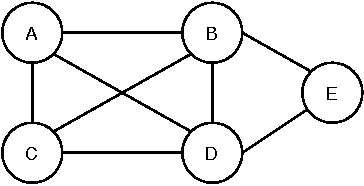
\includegraphics{Figures/graph.pdf}
	\caption{Diagrama de un grafo.}
	\label{fig:graph}
\end{figure}

En este grafo de ejemplo se encuentran los cliques con cardinalidad igual a 2 como se indican resaltado en negro en la figura \ref{fig:graph-cliques-2}.
\begin{figure}[H]
	\centering	
	\subfigure[Clique A-B]{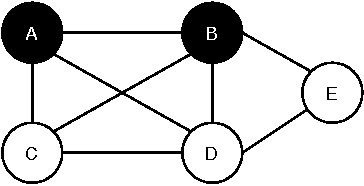
\includegraphics[width=0.275\textwidth]{Figures/graph-clique-AB.pdf}}
	\subfigure[Clique A-C]{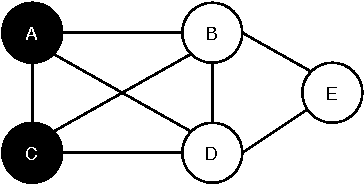
\includegraphics[width=0.275\textwidth]{Figures/graph-clique-AC.pdf}}
	\subfigure[Clique A-D]{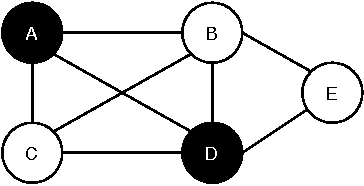
\includegraphics[width=0.275\textwidth]{Figures/graph-clique-AD.pdf}}
	\subfigure[Clique B-C]{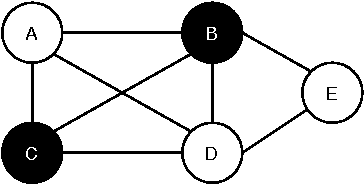
\includegraphics[width=0.275\textwidth]{Figures/graph-clique-BC.pdf}}
	\subfigure[Clique B-D]{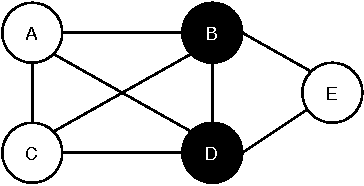
\includegraphics[width=0.275\textwidth]{Figures/graph-clique-BD.pdf}}
	\subfigure[Clique B-E]{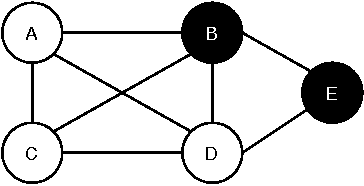
\includegraphics[width=0.275\textwidth]{Figures/graph-clique-BE.pdf}}
	\subfigure[Clique C-D]{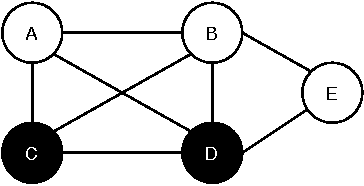
\includegraphics[width=0.275\textwidth]{Figures/graph-clique-CD.pdf}}
	\subfigure[Clique D-E]{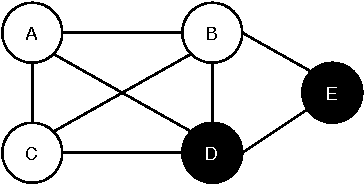
\includegraphics[width=0.275\textwidth]{Figures/graph-clique-DE.pdf}}
	\caption{Cliques de cardinalidad 2 del grafo.}
	\label{fig:graph-cliques-2}
\end{figure}
También se encuentran, como indica la figura \ref{fig:graph-cliques-3}, los cliques con cardinalidad igual a 3.
\begin{figure}[H]
	\centering	
	\subfigure[Clique A-B-C]{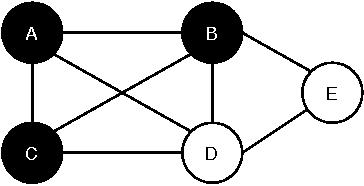
\includegraphics[width=0.275\textwidth]{Figures/graph-clique-ABC.pdf}}
	\subfigure[Clique A-B-D]{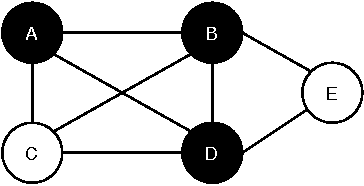
\includegraphics[width=0.275\textwidth]{Figures/graph-clique-ABD.pdf}}
	\subfigure[Clique A-C-D]{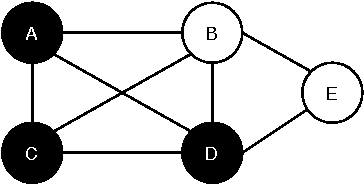
\includegraphics[width=0.275\textwidth]{Figures/graph-clique-ACD.pdf}}
	\subfigure[Clique B-C-D]{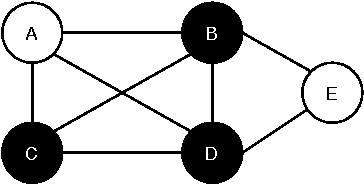
\includegraphics[width=0.275\textwidth]{Figures/graph-clique-BCD.pdf}}
	\subfigure[Clique B-D-E]{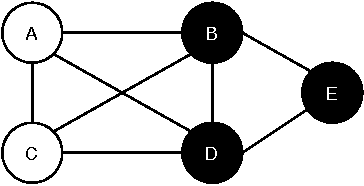
\includegraphics[width=0.275\textwidth]{Figures/graph-clique-BDE.pdf}}
	\caption{Cliques de cardinalidad 3 del grafo.}
	\label{fig:graph-cliques-3}
\end{figure}
Cabe destacar que los nodos, por si solos, también forman clique.

Una característica importante de un clique es que este puede ser máximo \cite{web-maximumclique}. Esto quiere decir que no se pueden añadir más nodos adyacentes que cumplan las restricciones necesarias para formar un clique, y a su vez, es el de mayor tamaño del grafo, como se muestra en la figura \ref{fig:max-clique}, a diferencia de un clique que se podría denominar simple  \cite{web-maximalclique}. 
\begin{figure}[H]
	\centering
	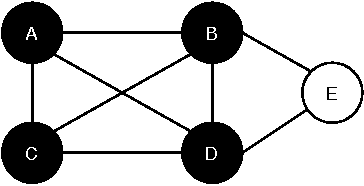
\includegraphics{Figures/graph-clique-max.pdf}
	\caption{Clique máximo del grafo.}
	\label{fig:max-clique}
\end{figure}
En este  caso, se obtiene $\omega(G) = 4$, donde $\omega$ denota el número de vértices del clique, su cardinalidad.

\section{Definición del problema}

\subsection{Problema del clique de ratio máximo}
\label{intro-problema}
Como se introdujo en la sección \ref{sec-clique}, el concepto clique es fundamental y muy estudiado, en concreto, la búsqueda del clique máximo dentro de un grafo. A este problema se le conoce como el problema del clique máximo o \gls{MCP} (Maximum clique problem), y es catalogado como un NP-completo.

En teoría de complejidad computacional, a los problemas denominados como NP, acrónimo de non-deterministic polynomial time o tiempo polinomial no determinista, se les conoce como el conjunto de problemas que se pueden resolver en un tiempo polinómico por una máquina de Turing no determinista. Esta clasificación, como se muestra en la figura \ref{fig:problemas-np}, también contiene todos los problemas de tipo P y de tipo NP-completos, como es el caso del problema del clique máximo.

\begin{figure}[H]
	\centering
	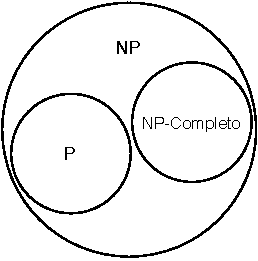
\includegraphics{Figures/problemas-np.pdf}
	\caption{Diagrama de problemas NP.}
	\label{fig:problemas-np}
\end{figure}

Una variante de este problema es el llamado problema del clique de peso máximo o \gls{MWCP} (Maximum Weight Clique Problem), en el que se asocia un peso no negativo a cada vértice, y cuyo objetivo es encontrar un clique con el máximo valor en la suma de los pesos de sus vértices.\\
Otra variante, la tratada en este trabajo, es el problema del clique de ratio máximo o \gls{MRCP} (Maximum Ratio Clique Problem) que trata de encontrar el subgrafo completo de ratio máximo. Este ratio se define como la proporción de la suma de los pesos no negativos asociados a los vértices del grafo como se indica a continuación:
\begin{equation*}
\frac{\sum_{i=1}^{n}p_ix_i}{\sum_{i=1}^{n}q_ix_i}
\end{equation*}
donde $p$ y $q$ son pesos no negativos asociados a cada vértice $i$, y $x$ se determina como:
\[
\diagram{$x_i=$}{
	1: si el vértice $i$ forma parte de la solución. \\
	0: en otro caso
}
\]

Como se expone en el modelo de ecuación \ref{eq:mrcp-max}, partiendo de un grafo simple no dirigido $G=(V, E)$, donde $V$ se asocia al conjunto de vértices pertenecientes al grafo, $\{v_1,\dots,v_n\}$, y $E$ es el conjunto de aristas que conectan los vértices del grafo, $\{(v_i,~v_j)\}$ tal que $i \neq j$ y $v_i,~v_j~\in V$, y suponiendo que los pesos asociados a cada vértice son positivos, se obtiene un clique máximo $\widehat{S}$, siempre y cuando se cumplan las restricciones \ref{eq:mrcp-rest1} - \ref{eq:mrcp-rest3}.

\begin{eqnarray}
\label{eq:mrcp-max} 
maximizar && f = \frac{\sum_{i=1}^{n}p_ix_i}{\sum_{i=1}^{n}q_ix_i} \\
\nonumber sujeto ~ a: \\
\label{eq:mrcp-rest1}
&& x_i + x_j \leqslant 1: \forall (v_i, v_j) \notin E,~i \neq j,\\
\label{eq:mrcp-rest2}
&& \sum_{i=1}^{n}(a_ij)x_i ~ \geqslant 1: \forall v_j \in V, \\
\label{eq:mrcp-rest3}
&& x_i \in {0,~1}: \forall v_i \in V.
\end{eqnarray}

El problema del clique de ratio máximo ha sido catalogado como un problema NP-difícil o NP-complejo como se indica en la figura \ref{fig:np-dificil}, por lo que no es posible obtener una solución factible por métodos heurísticos o exactos.

\begin{figure}[H]
	\centering
	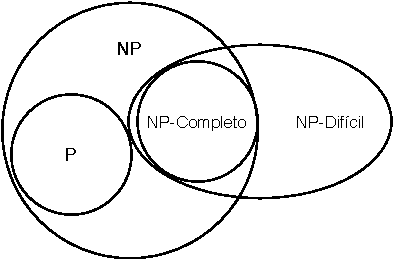
\includegraphics{Figures/problemas-np-hard.pdf}
	\caption{MRCP clasificado en los problemas NP-difícil.}
	\label{fig:np-dificil}
\end{figure}

\section{Estado del arte}
Si bien es cierto que no existe demasiada literatura al respecto, ya que se trata de un problema poco estudiado en comparación con el clásico problema de búsqueda de la clique máxima, \cite{mcp-batsyn}, \cite{mcp-ryp}, \cite{mcp-neuro}, o \cite{mcp-ants}, este análisis, y todo lo que rodea al mismo, ha sido documentado mediante la literatura que se explica a continuación. 

Un estudio muy cercano al tratado en este trabajo es el problema de la búsqueda del clique de peso máximo, en \cite{mwcp-ls} y \cite{mwcp-ml} se implementan algoritmos de búsqueda local, llamados SCCWalk y SCCWalk4L, en los que se hace uso del muestreo no determinista y el machine-learning para abordar el problema, eliminando variables de decisión que no formarían parte de una solución óptima.

En el documento desarrollado por Samyukta Sethuraman y Sergiy Butenko \cite{mrcp-Sethuraman:2015} se trata el problema desde tres puntos de vista, mediante el IBM CPLEX, para resolver el problema de manera lineal, la aplicación de la búsqueda binaria y el método de Newton.

En \cite{mrcp-moeni} se trata el problema basándose en el enfoque eficiente que dan las funciones de diferencia de convexos (DC) y sus algoritmos (DCA), que proveen resultados competitivos y a su vez introducen las desigualdades válidas, que ayudan a mejorar el tiempo computacional en la obtención de resultados de calidad al problema.

Cabe destacar entre todos los trabajos el de Dominik Goeke, Mahdi Moeini y David Poganiuch \cite{mrcp-GOEKE2017283} el cual se ha tomado como referencia para realizar este trabajo. En este artículo, los autores parten de un punto de vista multi-arranque \gls{MSM}, añadiendo una búsqueda de vecindario variable \gls{VNS}, lo que permite obtener soluciones de gran calidad con un tiempo de computo menor.

%-------------------------------------------------------------------------------

